\documentclass{standalone}
\usepackage{tikz}
\usetikzlibrary{patterns, positioning}
\usepackage[sfdefault]{ClearSans} %% option 'sfdefault' activates Clear Sans as the default text font
\usepackage[T1]{fontenc}

\begin{document}
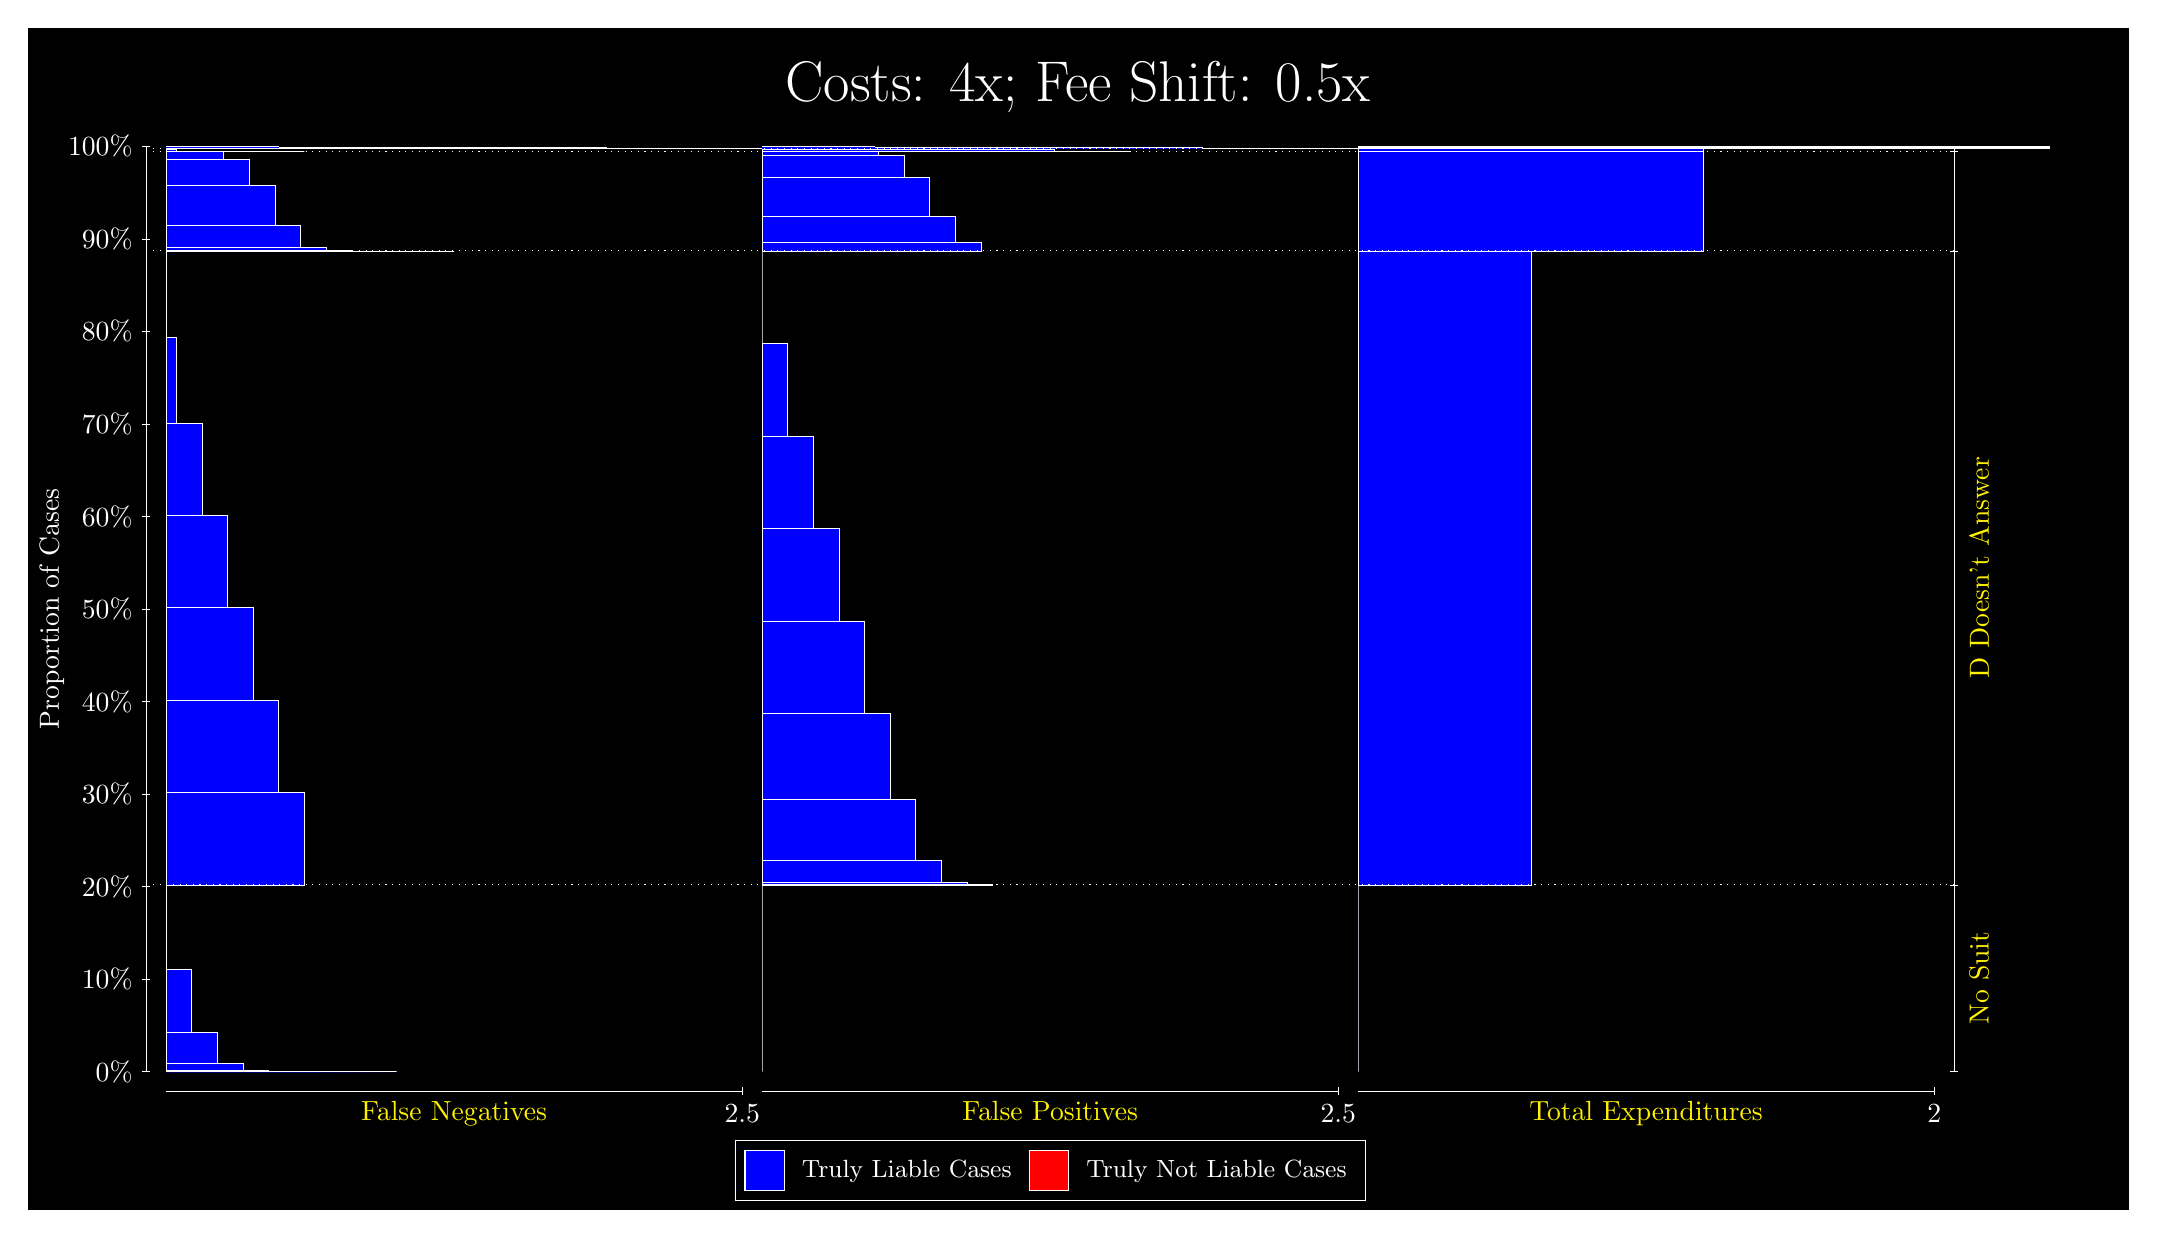
\begin{tikzpicture}
\draw[fill=black] (0,0) rectangle (26.667,15);
\draw[text=white] (0,13.5) rectangle (26.667,15) node[midway] {\huge Costs: 4x; Fee Shift: 0.5x};
\draw[white, very thin] (1.5,1.75) -- (1.5,13.5);
\node[rotate=90, text=white, anchor=center] at (0.3, 7.625) {Proportion of Cases};
\draw[white, very thin] (1.45,1.75) -- (1.55,1.75);
\node[text=white, anchor=east] at (1.45, 1.75) {0\%};
\draw[white, very thin] (1.45,2.925) -- (1.55,2.925);
\node[text=white, anchor=east] at (1.45, 2.925) {10\%};
\draw[white, very thin] (1.45,4.1) -- (1.55,4.1);
\node[text=white, anchor=east] at (1.45, 4.1) {20\%};
\draw[white, very thin] (1.45,5.275) -- (1.55,5.275);
\node[text=white, anchor=east] at (1.45, 5.275) {30\%};
\draw[white, very thin] (1.45,6.45) -- (1.55,6.45);
\node[text=white, anchor=east] at (1.45, 6.45) {40\%};
\draw[white, very thin] (1.45,7.625) -- (1.55,7.625);
\node[text=white, anchor=east] at (1.45, 7.625) {50\%};
\draw[white, very thin] (1.45,8.8) -- (1.55,8.8);
\node[text=white, anchor=east] at (1.45, 8.8) {60\%};
\draw[white, very thin] (1.45,9.975) -- (1.55,9.975);
\node[text=white, anchor=east] at (1.45, 9.975) {70\%};
\draw[white, very thin] (1.45,11.15) -- (1.55,11.15);
\node[text=white, anchor=east] at (1.45, 11.15) {80\%};
\draw[white, very thin] (1.45,12.325) -- (1.55,12.325);
\node[text=white, anchor=east] at (1.45, 12.325) {90\%};
\draw[white, very thin] (1.45,13.5) -- (1.55,13.5);
\node[text=white, anchor=east] at (1.45, 13.5) {100\%};

\draw[white, very thin] (24.457,1.75) -- (24.457,13.5);
\draw[white, very thin] (24.407,1.75) -- (24.507,1.75);
\node[anchor=west] at (24.407, 1.75) {};
\draw[white, very thin] (24.407,4.12) -- (24.507,4.12);
\node[anchor=west] at (24.407, 4.12) {};
\draw[white, very thin] (24.407,12.172) -- (24.507,12.172);
\node[anchor=west] at (24.407, 12.172) {};
\draw[white, very thin] (24.407,13.435) -- (24.507,13.435);
\node[anchor=west] at (24.407, 13.435) {};
\draw[white, very thin] (24.407,13.478) -- (24.507,13.478);
\node[anchor=west] at (24.407, 13.478) {};
\draw[white, very thin] (24.407,13.5) -- (24.507,13.5);
\node[anchor=west] at (24.407, 13.5) {};

\draw[white, very thin, fill=blue] (1.75,1.75) rectangle (4.6775,1.75);
\draw[white, very thin, fill=blue] (1.75,1.75) rectangle (4.3523,1.75);
\draw[white, very thin, fill=blue] (1.75,1.75) rectangle (4.027,1.75);
\draw[white, very thin, fill=blue] (1.75,1.75) rectangle (3.7017,1.75);
\draw[white, very thin, fill=blue] (1.75,1.75) rectangle (3.3764,1.7508);
\draw[white, very thin, fill=blue] (1.75,1.7508) rectangle (3.0511,1.7626);
\draw[white, very thin, fill=blue] (1.75,1.7626) rectangle (2.7258,1.8592);
\draw[white, very thin, fill=blue] (1.75,1.8592) rectangle (2.4006,2.2458);
\draw[white, very thin, fill=blue] (1.75,2.2458) rectangle (2.0753,3.0519);
\draw[white, very thin, fill=red] (1.75,3.0519) rectangle (1.75,3.0519);
\draw[white, very thin, fill=blue] (1.75,3.0519) rectangle (1.75,4.12);
\draw[white, very thin, fill=blue] (1.75,4.12) rectangle (3.5065,5.295);
\draw[white, very thin, fill=blue] (1.75,5.295) rectangle (3.1812,6.47);
\draw[white, very thin, fill=blue] (1.75,6.47) rectangle (2.856,7.645);
\draw[white, very thin, fill=blue] (1.75,7.645) rectangle (2.5307,8.8197);
\draw[white, very thin, fill=blue] (1.75,8.8197) rectangle (2.2054,9.9875);
\draw[white, very thin, fill=blue] (1.75,9.9875) rectangle (1.8801,11.081);
\draw[white, very thin, fill=red] (1.75,11.081) rectangle (1.75,11.081);
\draw[white, very thin, fill=blue] (1.75,11.081) rectangle (1.75,12.172);
\draw[white, very thin, fill=blue] (1.75,12.172) rectangle (5.4094,12.172);
\draw[white, very thin, fill=blue] (1.75,12.172) rectangle (5.0842,12.172);
\draw[white, very thin, fill=blue] (1.75,12.172) rectangle (4.7589,12.172);
\draw[white, very thin, fill=blue] (1.75,12.172) rectangle (4.4336,12.172);
\draw[white, very thin, fill=blue] (1.75,12.172) rectangle (4.1083,12.174);
\draw[white, very thin, fill=blue] (1.75,12.174) rectangle (3.783,12.22);
\draw[white, very thin, fill=blue] (1.75,12.22) rectangle (3.4577,12.497);
\draw[white, very thin, fill=blue] (1.75,12.497) rectangle (3.1325,12.999);
\draw[white, very thin, fill=blue] (1.75,12.999) rectangle (2.8072,13.331);
\draw[white, very thin, fill=blue] (1.75,13.331) rectangle (2.4819,13.435);
\draw[white, very thin, fill=red] (1.75,13.435) rectangle (1.75,13.435);
\draw[white, very thin, fill=blue] (1.75,13.435) rectangle (3.5065,13.435);
\draw[white, very thin, fill=blue] (1.75,13.435) rectangle (3.1812,13.435);
\draw[white, very thin, fill=blue] (1.75,13.435) rectangle (2.856,13.435);
\draw[white, very thin, fill=blue] (1.75,13.435) rectangle (2.5307,13.436);
\draw[white, very thin, fill=blue] (1.75,13.436) rectangle (2.2054,13.439);
\draw[white, very thin, fill=blue] (1.75,13.439) rectangle (1.8801,13.457);
\draw[white, very thin, fill=red] (1.75,13.457) rectangle (1.75,13.457);
\draw[white, very thin, fill=blue] (1.75,13.457) rectangle (1.75,13.478);
\draw[white, very thin, fill=blue] (1.75,13.478) rectangle (9.9471,13.478);
\draw[white, very thin, fill=blue] (1.75,13.478) rectangle (9.6218,13.478);
\draw[white, very thin, fill=blue] (1.75,13.478) rectangle (9.2966,13.478);
\draw[white, very thin, fill=blue] (1.75,13.478) rectangle (8.9713,13.478);
\draw[white, very thin, fill=blue] (1.75,13.478) rectangle (8.9713,13.478);
\draw[white, very thin, fill=blue] (1.75,13.478) rectangle (8.646,13.478);
\draw[white, very thin, fill=blue] (1.75,13.478) rectangle (8.3207,13.478);
\draw[white, very thin, fill=blue] (1.75,13.478) rectangle (8.3207,13.478);
\draw[white, very thin, fill=blue] (1.75,13.478) rectangle (7.9954,13.478);
\draw[white, very thin, fill=blue] (1.75,13.478) rectangle (7.9954,13.479);
\draw[white, very thin, fill=blue] (1.75,13.479) rectangle (7.6702,13.481);
\draw[white, very thin, fill=blue] (1.75,13.481) rectangle (7.3449,13.483);
\draw[white, very thin, fill=blue] (1.75,13.483) rectangle (7.3449,13.486);
\draw[white, very thin, fill=blue] (1.75,13.486) rectangle (7.0196,13.49);
\draw[white, very thin, fill=blue] (1.75,13.49) rectangle (6.6943,13.491);
\draw[white, very thin, fill=blue] (1.75,13.491) rectangle (6.369,13.491);
\draw[white, very thin, fill=blue] (1.75,13.491) rectangle (6.369,13.491);
\draw[white, very thin, fill=blue] (1.75,13.491) rectangle (6.0437,13.491);
\draw[white, very thin, fill=blue] (1.75,13.491) rectangle (5.1329,13.491);
\draw[white, very thin, fill=blue] (1.75,13.491) rectangle (4.8077,13.491);
\draw[white, very thin, fill=blue] (1.75,13.491) rectangle (4.4824,13.491);
\draw[white, very thin, fill=blue] (1.75,13.491) rectangle (4.4824,13.491);
\draw[white, very thin, fill=blue] (1.75,13.491) rectangle (4.1571,13.491);
\draw[white, very thin, fill=blue] (1.75,13.491) rectangle (3.8318,13.491);
\draw[white, very thin, fill=blue] (1.75,13.491) rectangle (3.8318,13.491);
\draw[white, very thin, fill=blue] (1.75,13.491) rectangle (3.5065,13.493);
\draw[white, very thin, fill=blue] (1.75,13.493) rectangle (3.1812,13.493);
\draw[white, very thin, fill=blue] (1.75,13.493) rectangle (3.1812,13.495);
\draw[white, very thin, fill=blue] (1.75,13.495) rectangle (3.1812,13.497);
\draw[white, very thin, fill=blue] (1.75,13.497) rectangle (2.856,13.498);
\draw[white, very thin, fill=blue] (1.75,13.498) rectangle (2.856,13.499);
\draw[white, very thin, fill=blue] (1.75,13.499) rectangle (2.5307,13.499);
\draw[white, very thin, fill=blue] (1.75,13.499) rectangle (2.5307,13.499);
\draw[white, very thin, fill=blue] (1.75,13.499) rectangle (2.5307,13.5);
\draw[white, very thin, fill=blue] (1.75,13.5) rectangle (2.2054,13.5);
\draw[white, very thin, fill=blue] (1.75,13.5) rectangle (2.2054,13.5);
\draw[white, very thin, fill=blue] (1.75,13.5) rectangle (1.8801,13.5);
\draw[white, very thin, fill=blue] (1.75,13.5) rectangle (1.8801,13.5);
\draw[white, very thin, fill=red] (1.75,13.5) rectangle (1.75,13.5);
\draw[white, very thin, fill=blue] (1.75,13.5) rectangle (1.75,13.5);
\draw[white, very thin, fill=red] (9.3189,1.75) rectangle (9.3189,1.75);
\draw[white, very thin, fill=blue] (9.3189,1.75) rectangle (9.3189,4.12);
\draw[white, very thin, fill=red] (9.3189,4.12) rectangle (12.246,4.12);
\draw[white, very thin, fill=blue] (9.3189,4.12) rectangle (12.246,4.122);
\draw[white, very thin, fill=blue] (9.3189,4.122) rectangle (11.921,4.1589);
\draw[white, very thin, fill=blue] (9.3189,4.1589) rectangle (11.596,4.437);
\draw[white, very thin, fill=blue] (9.3189,4.437) rectangle (11.271,5.2115);
\draw[white, very thin, fill=blue] (9.3189,5.2115) rectangle (10.945,6.3046);
\draw[white, very thin, fill=blue] (9.3189,6.3046) rectangle (10.62,7.4724);
\draw[white, very thin, fill=blue] (9.3189,7.4724) rectangle (10.295,8.6471);
\draw[white, very thin, fill=blue] (9.3189,8.6471) rectangle (9.9694,9.8221);
\draw[white, very thin, fill=blue] (9.3189,9.8221) rectangle (9.6442,10.997);
\draw[white, very thin, fill=blue] (9.3189,10.997) rectangle (9.3189,12.172);
\draw[white, very thin, fill=red] (9.3189,12.172) rectangle (12.1,12.172);
\draw[white, very thin, fill=blue] (9.3189,12.172) rectangle (12.1,12.277);
\draw[white, very thin, fill=blue] (9.3189,12.277) rectangle (11.775,12.608);
\draw[white, very thin, fill=blue] (9.3189,12.608) rectangle (11.449,13.111);
\draw[white, very thin, fill=blue] (9.3189,13.111) rectangle (11.124,13.387);
\draw[white, very thin, fill=blue] (9.3189,13.387) rectangle (10.799,13.434);
\draw[white, very thin, fill=blue] (9.3189,13.434) rectangle (10.474,13.435);
\draw[white, very thin, fill=blue] (9.3189,13.435) rectangle (10.148,13.435);
\draw[white, very thin, fill=blue] (9.3189,13.435) rectangle (9.8231,13.435);
\draw[white, very thin, fill=blue] (9.3189,13.435) rectangle (9.4978,13.435);
\draw[white, very thin, fill=blue] (9.3189,13.435) rectangle (9.3189,13.435);
\draw[white, very thin, fill=red] (9.3189,13.435) rectangle (14.003,13.435);
\draw[white, very thin, fill=blue] (9.3189,13.435) rectangle (14.003,13.435);
\draw[white, very thin, fill=blue] (9.3189,13.435) rectangle (13.678,13.436);
\draw[white, very thin, fill=blue] (9.3189,13.436) rectangle (13.352,13.439);
\draw[white, very thin, fill=blue] (9.3189,13.439) rectangle (13.027,13.457);
\draw[white, very thin, fill=blue] (9.3189,13.457) rectangle (12.702,13.474);
\draw[white, very thin, fill=blue] (9.3189,13.474) rectangle (12.377,13.478);
\draw[white, very thin, fill=blue] (9.3189,13.478) rectangle (12.051,13.478);
\draw[white, very thin, fill=blue] (9.3189,13.478) rectangle (11.726,13.478);
\draw[white, very thin, fill=blue] (9.3189,13.478) rectangle (11.401,13.478);
\draw[white, very thin, fill=blue] (9.3189,13.478) rectangle (11.075,13.478);
\draw[white, very thin, fill=red] (9.3189,13.478) rectangle (17.516,13.478);
\draw[white, very thin, fill=blue] (9.3189,13.478) rectangle (17.516,13.478);
\draw[white, very thin, fill=red] (9.3189,13.478) rectangle (17.191,13.478);
\draw[white, very thin, fill=blue] (9.3189,13.478) rectangle (17.191,13.478);
\draw[white, very thin, fill=red] (9.3189,13.478) rectangle (16.865,13.478);
\draw[white, very thin, fill=blue] (9.3189,13.478) rectangle (16.865,13.478);
\draw[white, very thin, fill=red] (9.3189,13.478) rectangle (16.54,13.478);
\draw[white, very thin, fill=blue] (9.3189,13.478) rectangle (16.54,13.478);
\draw[white, very thin, fill=red] (9.3189,13.478) rectangle (16.215,13.478);
\draw[white, very thin, fill=blue] (9.3189,13.478) rectangle (16.215,13.478);
\draw[white, very thin, fill=red] (9.3189,13.478) rectangle (15.89,13.478);
\draw[white, very thin, fill=blue] (9.3189,13.478) rectangle (15.89,13.478);
\draw[white, very thin, fill=blue] (9.3189,13.478) rectangle (15.89,13.478);
\draw[white, very thin, fill=blue] (9.3189,13.478) rectangle (15.564,13.478);
\draw[white, very thin, fill=blue] (9.3189,13.478) rectangle (15.564,13.479);
\draw[white, very thin, fill=blue] (9.3189,13.479) rectangle (15.239,13.48);
\draw[white, very thin, fill=blue] (9.3189,13.48) rectangle (15.239,13.481);
\draw[white, very thin, fill=blue] (9.3189,13.481) rectangle (14.914,13.484);
\draw[white, very thin, fill=blue] (9.3189,13.484) rectangle (14.914,13.484);
\draw[white, very thin, fill=blue] (9.3189,13.484) rectangle (14.914,13.485);
\draw[white, very thin, fill=blue] (9.3189,13.485) rectangle (14.588,13.487);
\draw[white, very thin, fill=blue] (9.3189,13.487) rectangle (14.588,13.487);
\draw[white, very thin, fill=blue] (9.3189,13.487) rectangle (14.588,13.487);
\draw[white, very thin, fill=blue] (9.3189,13.487) rectangle (14.263,13.487);
\draw[white, very thin, fill=blue] (9.3189,13.487) rectangle (14.263,13.487);
\draw[white, very thin, fill=blue] (9.3189,13.487) rectangle (13.938,13.487);
\draw[white, very thin, fill=blue] (9.3189,13.487) rectangle (13.938,13.487);
\draw[white, very thin, fill=blue] (9.3189,13.487) rectangle (13.613,13.487);
\draw[white, very thin, fill=blue] (9.3189,13.487) rectangle (13.613,13.487);
\draw[white, very thin, fill=blue] (9.3189,13.487) rectangle (13.287,13.487);
\draw[white, very thin, fill=blue] (9.3189,13.487) rectangle (13.287,13.487);
\draw[white, very thin, fill=blue] (9.3189,13.487) rectangle (12.962,13.487);
\draw[white, very thin, fill=red] (9.3189,13.487) rectangle (12.051,13.487);
\draw[white, very thin, fill=blue] (9.3189,13.487) rectangle (12.051,13.487);
\draw[white, very thin, fill=red] (9.3189,13.487) rectangle (11.726,13.487);
\draw[white, very thin, fill=blue] (9.3189,13.487) rectangle (11.726,13.487);
\draw[white, very thin, fill=blue] (9.3189,13.487) rectangle (11.401,13.488);
\draw[white, very thin, fill=red] (9.3189,13.488) rectangle (11.401,13.488);
\draw[white, very thin, fill=blue] (9.3189,13.488) rectangle (11.401,13.488);
\draw[white, very thin, fill=blue] (9.3189,13.488) rectangle (11.075,13.491);
\draw[white, very thin, fill=red] (9.3189,13.491) rectangle (11.075,13.491);
\draw[white, very thin, fill=blue] (9.3189,13.491) rectangle (11.075,13.492);
\draw[white, very thin, fill=blue] (9.3189,13.492) rectangle (11.075,13.492);
\draw[white, very thin, fill=blue] (9.3189,13.492) rectangle (10.75,13.494);
\draw[white, very thin, fill=blue] (9.3189,13.494) rectangle (10.75,13.496);
\draw[white, very thin, fill=blue] (9.3189,13.496) rectangle (10.75,13.497);
\draw[white, very thin, fill=blue] (9.3189,13.497) rectangle (10.425,13.498);
\draw[white, very thin, fill=blue] (9.3189,13.498) rectangle (10.425,13.499);
\draw[white, very thin, fill=blue] (9.3189,13.499) rectangle (10.1,13.499);
\draw[white, very thin, fill=blue] (9.3189,13.499) rectangle (10.1,13.5);
\draw[white, very thin, fill=blue] (9.3189,13.5) rectangle (10.1,13.5);
\draw[white, very thin, fill=blue] (9.3189,13.5) rectangle (9.7743,13.5);
\draw[white, very thin, fill=blue] (9.3189,13.5) rectangle (9.7743,13.5);
\draw[white, very thin, fill=blue] (9.3189,13.5) rectangle (9.449,13.5);
\draw[white, very thin, fill=blue] (9.3189,13.5) rectangle (9.449,13.5);
\draw[white, very thin, fill=blue] (9.3189,13.5) rectangle (9.3189,13.5);
\draw[white, very thin, fill=red] (16.888,1.75) rectangle (16.888,1.75);
\draw[white, very thin, fill=blue] (16.888,1.75) rectangle (16.888,4.12);
\draw[white, very thin, fill=red] (16.888,4.12) rectangle (19.083,4.12);
\draw[white, very thin, fill=blue] (16.888,4.12) rectangle (19.083,12.172);
\draw[white, very thin, fill=red] (16.888,12.172) rectangle (21.279,12.172);
\draw[white, very thin, fill=blue] (16.888,12.172) rectangle (21.279,13.435);
\draw[white, very thin, fill=red] (16.888,13.435) rectangle (21.279,13.435);
\draw[white, very thin, fill=blue] (16.888,13.435) rectangle (21.279,13.478);
\draw[white, very thin, fill=red] (16.888,13.478) rectangle (25.67,13.478);
\draw[white, very thin, fill=blue] (16.888,13.478) rectangle (25.67,13.489);
\draw[white, very thin, fill=red] (16.888,13.489) rectangle (25.67,13.489);
\draw[white, very thin, fill=blue] (16.888,13.489) rectangle (25.67,13.5);
\draw[white, dotted] (1.5,4.12) -- (24.457,4.12);
\draw[white, dotted] (1.5,12.172) -- (24.457,12.172);
\draw[white, dotted] (1.5,13.435) -- (24.457,13.435);
\draw[white, dotted] (1.5,13.478) -- (24.457,13.478);
\draw[white, very thin] (1.75,1.5) -- (9.0689,1.5);
\node[text=yellow, anchor=north] at (5.4094, 1.5) {False Negatives};
\draw[white, very thin] (9.0689,1.45) -- (9.0689,1.55);
\node[text=white, anchor=north] at (9.0689, 1.45) {2.5};

\draw[white, very thin] (9.3189,1.5) -- (16.638,1.5);
\node[text=yellow, anchor=north] at (12.978, 1.5) {False Positives};
\draw[white, very thin] (16.638,1.45) -- (16.638,1.55);
\node[text=white, anchor=north] at (16.638, 1.45) {2.5};

\draw[white, very thin] (16.888,1.5) -- (24.207,1.5);
\node[text=yellow, anchor=north] at (20.547, 1.5) {Total Expenditures};
\draw[white, very thin] (24.207,1.45) -- (24.207,1.55);
\node[text=white, anchor=north] at (24.207, 1.45) {2};

\node[text=yellow, centered, rotate=90] at (24.777, 2.935) {No Suit};
\node[text=yellow, centered, rotate=90] at (24.777, 8.1461) {D Doesn't Answer};




\draw (12.978300999999998,1.5) node[draw=none] (baseCoordinate) {};
\begin{scope}[align=center]
        \matrix[scale=0.5, draw=white, below=0.5cm of baseCoordinate, nodes={draw}, column sep=0.1cm]{
            \node[rectangle, draw, minimum width=0.5cm, minimum height=0.5cm, fill=blue] {}; &
            \node[draw=none, font=\small, text=white] (B) {Truly Liable Cases}; &
            \node[rectangle, draw, minimum width=0.5cm, minimum height=0.5cm, fill=red] {}; &
            \node[draw=none, font=\small, text=white] (B) {Truly Not Liable Cases}; \\
            };
\end{scope}

\end{tikzpicture}
\end{document}